\documentclass[a4paper]{article}
\usepackage[T1]{fontenc}
\usepackage[utf8x]{inputenc}
\usepackage[italian]{babel}
\usepackage{graphicx}
\usepackage{amsmath}
\numberwithin{equation}{section}% numera eq come #section.#formula
\usepackage{amsthm}
\usepackage{amssymb}
\usepackage{cancel}
\usepackage{subfigure}
\usepackage{mathtools}
\usepackage{esint}
\usepackage{float}
 \usepackage{import}
\usepackage{xcolor}
\usepackage{geometry}
\geometry{a4paper, top=2cm, bottom=2cm, left=2.5cm, right=2.5cm,  heightrounded, bindingoffset=5mm}
\setlength{\parindent}{0pt} %riduce l'indentazione dei paragrafi
% Quanto segue serve per inserire l'elenco di equazioni
\usepackage[subfigure]{tocloft}
 \newcommand{\listequationsname}{Elenco delle equazioni}
\newlistof{myequations}{equ}{\listequationsname}
\newcommand{\myequations}[1]{%
	\addcontentsline{equ}{myequations}{\protect\numberline{\theequation}#1}\par}
% aggiungere per ogni etichetta oltre \label anche \myequations{NOME}
\setlength{\cftmyequationsnumwidth}{2.3em}
\setlength{\cftmyequationsindent}{1.5em}


\usepackage{makeidx} %serve per fare l'indice analitico
% compilare il documento principale
% viene generato un file nome_file.idx
% aprire il file e andare su Strumenti -> Comandi -> \makeindex
% compilare nuovamente il documento iniziale
\makeindex
% aggiungere gli elementi con \index{NOME}
% \index{Voce ! Voce secondaria}

\renewcommand{\thesubsubsection}{}
%rimuove la numerazione dalle sotto-sotto sezione

\title{Formulario fisica tecnica}
\author{
	Mastrofini Alessandro\\
	\and
	Volpato Rebecca\\
}
\date{October 2021}

\begin{document}

\newpage
\maketitle
\newpage
\tableofcontents
\newpage	

\newpage 

Novità rispetto al programma:
\begin{itemize}
	\item Al posto degli esercizi sulla trasmissione del calore verranno raccontate alcune esperienze.
	\item 	\textbf{Orale}: tre domande di teoria (termodinamica, termofluidodinamica, termocinetica o trasporto di massa) 
	\item \textbf{Scritto}: due esercitazioni, una sulle miscele aria-vapore (studio del benessere ambientale, saper regolare ambienti in ambienti clinici), cicli frigoriferi, terza domanda semi teorica (raccontare una delle esercitazioni citate sopra). 
	\item Esercitazioni sulla criochirurgia, sulla termoregolazione del corpo umano, sul trasporto di massa in aorta aneurismatica, sul trasporto di massa nel circolo di Willis e sull’acustica ovvero rumore provocato dalle valvole stenotiche. 
	\item Non ci sono esercizi sulla trasmissione del calore e termofluidodinamica.
	\item Testo: Problematiche di fisica tecnica in ingegneria medica (9 capitoli, da Texmat). Risultati di lavori fatti da colleghi o in tesi di dottorato o nella tesi magistrale ecc.
	
\end{itemize}


\newpage 


\section{Termodinamica}
	 \index{Termodinamica}
\subsection{Introduzione}
	
parliamo delle termodinamica classica $\rightarrow$ Ottocentesca


La prima cosa che bisogna fare nella termodinamica classica è definire l’oggetto del nostro studio, cioè l’insieme dei corpi che vogliamo studiare e che chiameremo \textcolor{red}{sistema termodinamico} (insieme degli oggetti che vogliamo studiare), si decide quale sistema termodinamico si vuole studiare, ad esempio l’aria nella stanza.
Nel momento in cui decidiamo il sistema, decidiamo anche il contorno fisico del nostro sistema termodinamico S scelto arbitrariamente; quello che c’è all’interno del nostro sistema è l’oggetto del nostro studio, tutto il resto è l’esterno E, mentre S è all’interno del contorno fisico.
\textbf{Sistema termodinamico} : oggetto del nostro studio.
Vogliamo relazionare il sistema termodinamico, cioè quello che c’è all’interno, con l’esterno e in particolare ci interessa la relazione, ovvero le interazioni tra l’interno e l’esterno, cioè ci interessa quello che succede NEL sistema.

Consideriamo tre tipologie di scambi:
\begin{itemize}
	\item Scambi di massa (sistemi aperti)
	\item Scambi di lavoro (attraverso il contorno)
	\item Scambi di calore (attraverso il contorno)
\end{itemize}

Individuiamo quindi lo stato termodinamico del sistema univocamente con:
\begin{itemize}
	\item $M$, composizione chimica
	\item $p,v,T$ , variabili interne 
	\item $w,z$, variabili esterne (velocità e quota)
\end{itemize}

Sono ipotesi lontane dalla realtà poiché la termodinamica classica studia \underline{solo stati di equilibrio}. 


 
 \index{Lavoro}
Definizione fisica del \textbf{lavoro}: si parte dal sistema cilindro-pistone \begin{equation}
	l_i=\int_1^2 p_idv
\end{equation}
\label{lavoro}
\myequations{Lavoro}  

Lo so definisce a partire dal sistema cilindro-pistone al quale applichiamo una forza $F$. 

\textbf{Convenzione termodinamica}: lavoro positivo se fatto dal sistema verso l'esterno.

\textbf{Convenzione termodinamica}: calore positivo se assorbito dal sistema (convezione opposta al lavoro).

Ricordiamo che siamo in uno stato di equilibrio, ovvero il caso limite. 

Nell'esempio del palloncino affinché possa aumentare il volume dovremo essere nelle condizioni in cui il lavoro di dilatazione è trascurabile, $l_i=l_e+\cancel{l_d}$. Questo è possibile quando:
\begin{itemize}
	\item c'è equilibrio termodinamico interno
	\item $p_i=p_e$, altrimenti la differenza di pressione dilata il materiale
	\item Assenza di attriti
	\item $T_i=T_e$
\end{itemize}

Queste condizioni non sono mai realizzabili, l’importanza della termodinamica però è che è una scienza che ragiona al limite; lo scopo dell’ingegneria è quello di dire vediamo di ridurre l’importanza di queste differenze di pressione tra interno ed esterno.


\textbf{Temperatura}: a partire dal termosocopio scegliamo una funzione che dipende da una delle variabili del sistema $\theta_A=f0(x)$ e nel sistema internazionale scegliamo una funzione lineare: $f'(x)=ax=T_A$. Quindi si dimostra che la \textbf{temperatura empirica} $\theta _A$ è uguale alla \textbf{temperatura termodinamica} $T_A$. Fissando il punto triplo dell'acqua $T_T=273.16 \text{K}$ eliminiamo la costante incognita  $rightarrow  T=273.16 {\over x_T}$. Usando il punti fisso del ghiaccio e il punto fisso del vapore $rightarrow T_{v}-T_{g}=a\left(x_{v}-x_{g}\right) \Rightarrow \frac{T}{T_{v}-T_{g}}=\frac{x}{x_{v}-x_{g}} $. Nel  S.I.$T\left({ }^{\circ} C\right)=T(K)-273,15$


\subsection{Misure}

Grande intensive --> minuscole
Grandezze intensive --> maiuscole

Misura della pressione 

Il barometro misura la pressione assoluta $p_A=\rho g h$

Manometro differenziale: dislivello => differenza di pressione. Bilancio delle forze : $ \rho S+\rho S\Delta z g=p_AS+\rho_m S\Delta z g$
 
Allora si ottiene che la pressione del fluido in esame rispetto la pressione atmosferica è $\rho -\rho_A=\rho_m \Delta zg$ 

\subsection{Frigoriferi ad effetto termoelettrico}


Permettono di misurare la temperatura. 

\textbf{Effetto Seebeck}

Presi due metalli saldati alle estremità. Mettendo le due saldature a T diverse misuriamo un forza elettromotrice $\Delta E=f\left(T_A-T_B\right)=\alpha_{A B}\left(T_{A}-\mathrm{T}_{B}\right) $ dove l coefficiente di Seebeck dipende dai materiali ed è definito come $\alpha_{A B}:=\lim _{\Delta T \rightarrow 0} \frac{\Delta E}{\Delta T}=\frac{d E}{d T}$. Usato nei dispositivi di misura: termocoppie. 

\begin{figure}[H]
	\begin{center}
		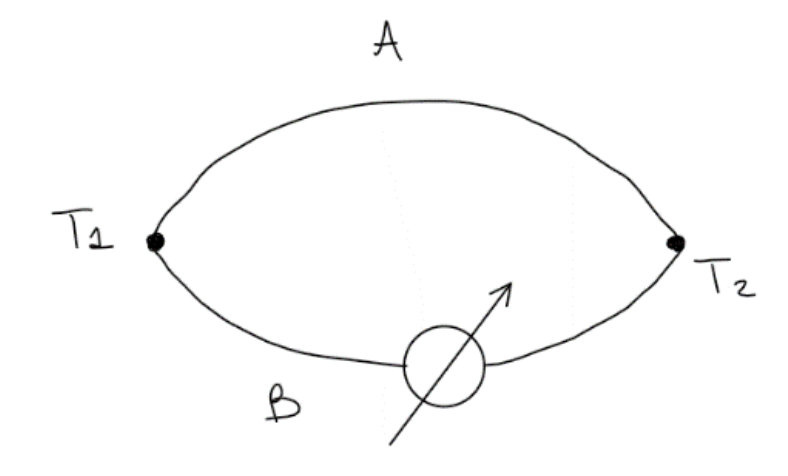
\includegraphics[width=0.2\columnwidth]{seebeck.png}
	\end{center}
\end{figure}

\textbf{Effetto Peltier} completa


\textbf{Effetto Thompson} 
Corrente in un conduttore metallico $\Longrightarrow$ differenza di temperatura. La quantità di calore che viene scambiata con l’esterno è in valore
assoluto proporzionale alla corrente, alla differenza di temperatura e ad un coefficiente che è chiamato coefficiente di Thomson.
$$\left|d \dot{Q}_{T}\right|=|\tau I d T|=\left|\tau I \frac{d T}{d x} d x\right|$$ 

\subsection{Principio zero della termodinamica}

\textbf{Principio zero della termodinamica} o di Fowler. Presi due corpi A in equilibrio con C tramite una parete conduttrice. E il corpo B in equilibrio con lo stesso C. Allora, essendo entrambi in equilibrio con C, saranno A in equilibrio con B. $\Longrightarrow$ Possiamo usare C come termoscopio, per misurare se due corpi sono in equilibrio termico. 

\textbf{calore}
È l’interazione tra il sistema termodinamico e l’esterno, che avviene a causa di una differenza di temperatura, attraverso il contorno (tanto all’interno c’è equilibrio e non mi interessa). Questa definizione è generale, c'è anche quella operativa. 

\subsection{Primo principio della termodinamica}
 \index{Primo principio}
Il primo principio della termodinamica stabilisce che il lavoro scambiato in una trasformazione termodinamica {\color{red}{ciclica}} in un sistema {\color{red}{chiuso}} è uguale al calore totale scambiato: 
\begin{equation}
	L=Q
\end{equation}		
\label{primoprincipio}
\myequations{Primo principio della termodinamica}
Ricorda Esperienza di Joule e il fatto che lavoro e calore sono sono negativi (lavoro assorbito e calore ceduto) $-|L|=-|Q|$

Generalizzando vale l'uguaglianza integrale e quindi $dQ-dL=dE$ nota come \textbf{energia totale} e si tratta di una funzione di stato infatti $\oint dE=0$.

L'energia totale dipende da variabili interne e variabili esterne. $E=E_{interne}+E_{esterne}$
Tra le variabili esterne troviamo:
\begin{itemize}
	\item velocità del baricentro
	\item quota del baricentro
\end{itemize}
Allora $\Delta E_e=\Delta E_c+\Delta E_p$ (energia cinetica e potenziale).

Tra le variabili interne troviamo:
\begin{itemize}
	\item variabili termodinamiche (pressione, volume specifico, temperatura)
	\item componenti elettrochimiche (reazioni chimiche, fenomeni elettrici o termoelettrici)
\end{itemize}
Allora $\Delta E_i=\Delta u+\Delta u_x$ (energia interna termodinamica e energia interna di origine elettrochimica).

\textbf{Primo principio della termodinamica per un sistema chiuso che compie trasformazioni aperte}: 
 \index{Primo principio! trasf aperte in un sistema chiuso}
\begin{equation}
	Q-L=\Delta u+\Delta E_c +\Delta E_p 
\end{equation}
\label{1principio}
\myequations{Primo principio}

In termini differenziali:
\begin{equation}
	dq-dl=du+du_x+{dw^2\over 2}+g dz 
\end{equation}
\label{1principiodiff}
\myequations{Primo principio in termini differenziali}
 
\begin{figure}[h!]
	\begin{center}
		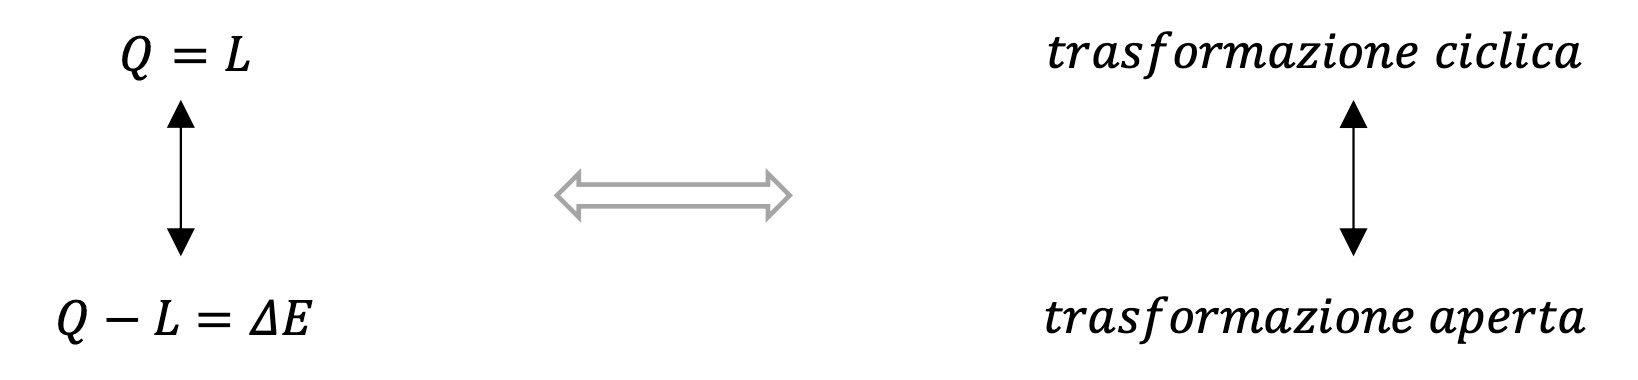
\includegraphics[width=0.6\columnwidth]{generalizprincipio.jpg}
	\end{center}
\end{figure}

\subsection{Sistemi aperti}
Lavoriamo in ipotesi di regime stazionario, in cui vale il bilancio di massa.
$M_t=M_{t+\Delta t}$
\begin{figure}[h!]
	\begin{center}
%		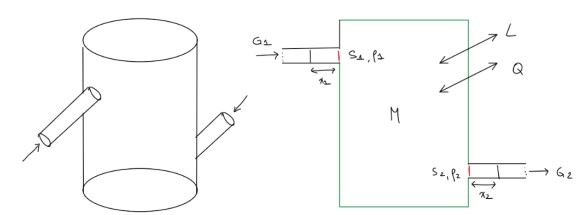
\includegraphics[width=0.6\columnwidth]{sistemaaperto.jpg}
		 \input{sistemaperto.pdf_tex}
	\end{center}
\end{figure}


\textbf{bilancio di energia} $q-l_f-p_2v_2+p_1v_1=\Delta u + \frac{\Delta w^2}{2}+g\Delta z$

Dall'equazione del bilancio dell'energia entra in gioco una nuova grandezza funzione di stato: \textbf{Entalpia}: $h=u+pv$

\begin{equation}
	q-l_f=\Delta h +\Delta e_c + \Delta e_p
\end{equation}
\myequations{Primo principio per sistemi aperti}
Si definisce Entalpia come il calore scambiato in un sistema aperto dove non è presente lavoro e non ci sono variazioni di energia cinetica e di energia potenziale. $dq=dh$

\subsubsection{Espansore}
È un sistema aperto per produrre lavoro verso l'esterno. Il fluido si espando, diminuisce la pressione $\longrightarrow$ lavoro positivo (vedi \eqref{eq:lavorosistemiaperti}). 
\begin{figure}[H]
	\begin{center}
		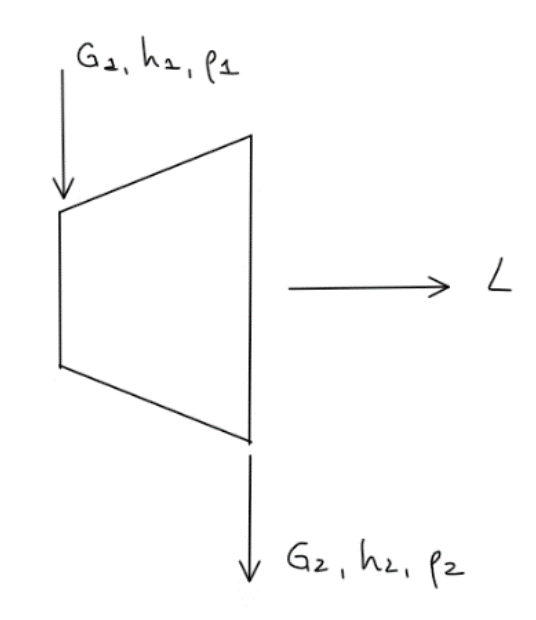
\includegraphics[width=0.2\columnwidth]{espansore.png}
	\end{center}
\end{figure}

Applichiamo il principio di conservazione della massa in regime stazionario e il principio di conservazione dell'energia (1° principio)  nel caso in cui $q=0$. Allora abbiamo \begin{equation}
	l_f=h_1-h_2>0
\end{equation}
\myequations{Lavoro dell'espansore}
Il fluido esce con un'entalpia minore. 

La potenza meccanica $P=l_f\cdot G_1=G\left(h_2-h_1\right)>0$

Il rendimento dell'espansore $\rho_{e}=\frac{l_{\text {reale }}}{l_{\text {ideale }}}=\frac{h_{1}-h_{2}}{\left(h_{1}-h_{2}\right)_{s}}$ , ha come limite superiore 1 (reversibilità). Nel caso ideale ($q=0$) consideriamo non ci siano cause di irreversibilità allora è una trasformazione adiabatica e reversibile $\Rightarrow$  isoentropica.

Quindi: $\rho_{e} \leq 1\begin{cases}
	=1 \text { per le trasformazioni reversibili } \\
	<1 \text { per le trasformazioni irreversibili reali }
\end{cases}$

\subsubsection{Compressore}

Con le stesse relazioni dell'espansore otteniamo un lavoro negativo (ceduto al sistema) 
\begin{equation}
	l_f=h_1-h_2<0
\end{equation}
\myequations{Lavoro del compressore}

\begin{figure}[H]
	\begin{center}
		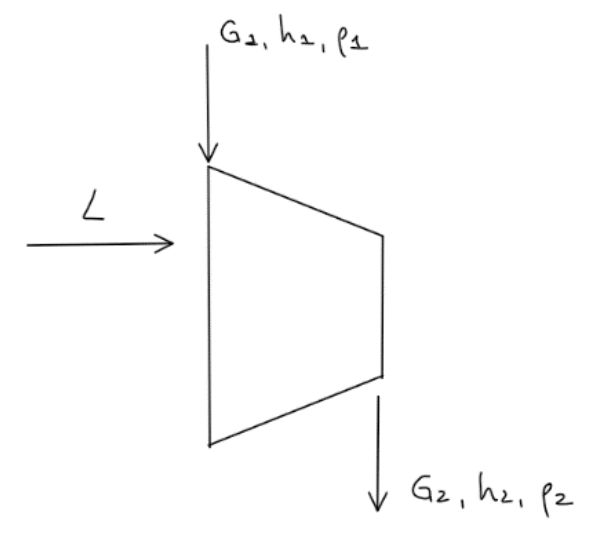
\includegraphics[width=0.2\columnwidth]{compressore.png}
	\end{center}
\end{figure}

C'è un aumento di entalpia dovuto al fatto che viene fornito lavoro al fluido $\Rightarrow$ aumento di pressione. $p_2>p_1$.

Analogamente per la potenza e il rendimento del compressore è il reciproco del rendimento dell'espansore. Il limite superiore è sempre 1 e valgono le stesse considerazioni dell'espansore. 

\subsubsection{Valvola di laminazione}

Non abbiamo scambi di calore ($q=0$) e $T_1=T_2$ e non c'è lavoro in quanto non c'è nessun organo meccanico che scambia lavoro. 

\begin{figure}[H]
	\begin{center}
				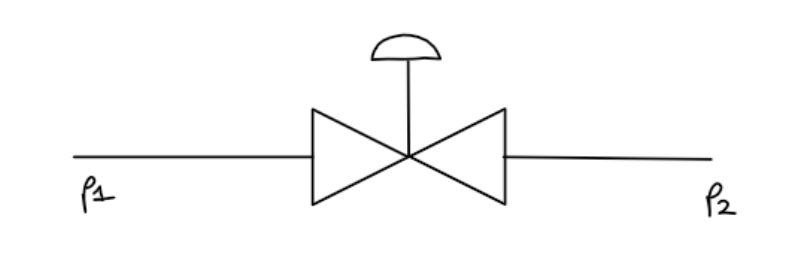
\includegraphics[width=0.3\columnwidth]{valvolalaminazione.png}
	\end{center}
\end{figure}

Allora dall'equazione del primo principio otteniamo
\begin{equation}
	\Delta h=0\Longrightarrow h_1=h_2
\end{equation}
\myequations{Valvola di laminazione}
È una tipica trasformazione \underline{irreversibile} poiché c'è un salto finito di pressione, cioè NON si parla di una trasformazione isoentalpica ma solo dell'uguglianza $h_1=h_2$. 

\subsubsection{Tubo di efflusso}

Riguarda la conversione dell'entalpia di un fluido in energia cinetica.

\begin{figure}[H]
	\begin{center}
		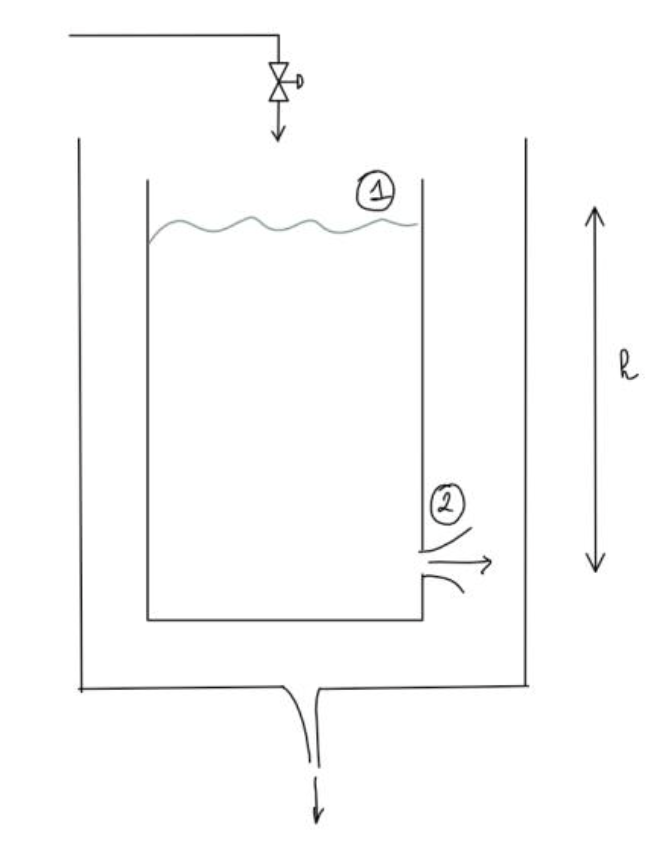
\includegraphics[width=0.3\columnwidth]{tuboefflusso.png}
	\end{center}
\end{figure}

Esperienza di Torricelli $\frac{w^{2}}{2 g}=h \rightarrow w=\sqrt{2 g h}$. 

Applicando il 1° principio (trascurando calore e lavoro) otteniamo $w_{2}^{2}=2 g\left(z_{1}-z_{2}\right)=2 g h$ da cui si torna al teorema di Torricelli.

\subsection{Calore}
\index{Calore}
\textbf{Definizione operativa}: il calore si misura come il lavoro scambiato da un sistema in un'esperienza di Joule. Ovvero un sistema chiuso che compie una trasformazione ciclica. 

\subsection{Secondo principio della termodinamica}
 \index{Secondo principio}
\textbf{Fromulazione di Plank}:
E' impossibile che l'unico risultato di una cessione di calore ad un sistema chiuso che compie trasformazioni cicliche sia la produzione di calore.

\textbf{Fromulazione di Clausius}:
E' impossibile che per un sistema chiuso che compie trasformazioni cicliche l'unico risultato sia la sottrazione di calore da una sorgente inferiore e la cessione di calore ad una sorgente superiore senza alcun effetto compensatorio.

\begin{figure}[H]
	\begin{center}
		\caption{Macchina di Newcomen}
		%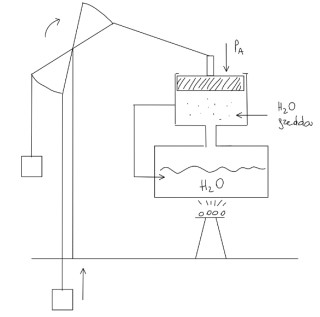
\includegraphics[width=0.4\columnwidth]{macchinaNewcomen.jpg}
				 \input{newcommen.pdf_tex}
	\end{center}
\end{figure}

Definiamo il rendimento come il rapporto tra ciò che si ottiene e ciò che si spende.
Questo meccanismo venne migliorato dalla macchina di Watt;

\begin{figure}[H]
	\begin{center}
		\caption{Macchina di Watt}
		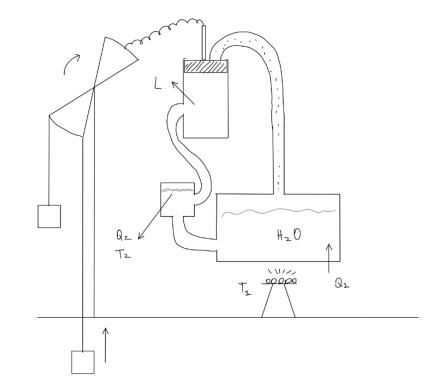
\includegraphics[width=0.6\columnwidth]{macchinadiWatt.jpg}
	\end{center}
\end{figure}

Distinguiamo il calore $Q_1$ che è il calore ceduto dal braciere al sistema termodinamico, il lavoro $L$ come il lavoro positivo esercitato dal sistema verso l'esterno e il calore $Q_2$ come il calore sottratto al sistema per ricondensare il vapore.

Per un sistema termodinamico chiuso che produce lavoro positivo grazie a scambi di calore il limite superiore del rendimento è il rendimento formulato da Carnot: $\eta_{max}=1-\frac{T_2}{T_1}$

\begin{figure}[H]
	\begin{center}
		\caption{Macchina motrice termica}
		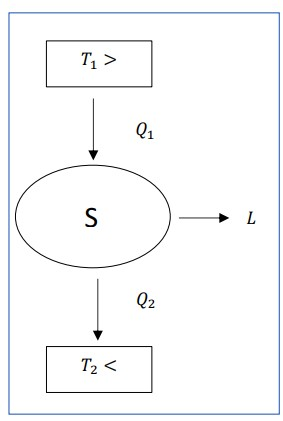
\includegraphics[width=0.2\columnwidth]{sistema.jpg}
	\end{center}
\end{figure}

Carnot fece una similitudine tra il mulino d'acqua e la macchina di Watt;
\begin{itemize}
	\item il lavoro L è lo stesso che produce in entrambi i casi una rotazione
	\item la quota coincide con la temperatura
	\item la portata coincide con il calore
\end{itemize}

il parallelismo errato era quello tra il calore e la portata perchè portava a scrivere $l=Q_1-Q_2=0$
Ma sappiamo che per produrre lavoro positivo la macchina di Watt deve avere $Q_1>Q_2$

Nei sistemi chiusi non si può invertire il segno del calore e del lavoro $\longrightarrow $ fenomeni sono \textbf{irreversibili}

\subsubsection{equivalenza dei principi}
 \index{Secondo principio! equivalenza}

\textbf{nego Plank}

\begin{figure}[H]
	\begin{center}
		\subfigure[Nego Plank]{
		\includegraphics[width=0.25\columnwidth]{Plank.jpg}}
		\subfigure[Nego Celsius]{
		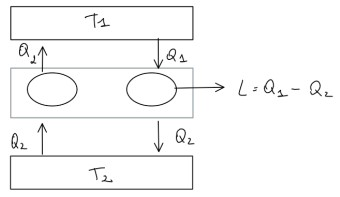
\includegraphics[width=0.4\columnwidth]{Clausius.jpg}}
	\end{center}
\end{figure}

\subsection{Equazioni del secondo principio}
 \index{Secondo principio! equazioni}
\begin{equation}
	\oint \frac{dQ}{T} \le 0
\end{equation}
\myequations{Disuguaglianza di Clausius}
Questa viene chiamata \textbf{Disuguaglianza di Clausius}; dove T è la temperatura alla quale si scambia calore $dQ$. La disuguaglianza è:
\begin{itemize}
	\item $=0$ per trasformazioni reversibili
	\item $<$ per trasformazioni irreversibili
\end{itemize}

La disuguaglianza di Clausius cambiata di segno è la \textbf{Traccia termodinamica}

\textbf{ciclo diretto}
$\frac{Q_1}{T_1} - \frac{Q_2}{T_2} \le 0 \longrightarrow \frac{Q_{ass}}{T_{ass}} \le \frac{Q_{ced}}{T_[ced]}$

\textbf{ciclo inverso}
$-\frac{Q_1}{T_1} + \frac{Q_2}{T_2} \le 0 \longrightarrow \frac{Q_{ass}}{T_{ass}} \le \frac{Q_{ced}}{T_[ced]}$

Consideriamo la macchina negata della formulazione di Plank e verifichiamo che la disuguaglianza di Clausius sia negata; poichè il calore assorbito è positivo la disuguaglianza di Clausius risulta negata.

\subsection{Entropia}
\index{Entropia}
per una trasformazione reversibile $\oint \frac{dQ}{T}=0$
allora la grandezza $\frac{dQ}{T}=ds$: \textbf{Entropia}

se la trasformazione è irreversibile $\oint\frac{dQ}{T} \le 0$ e quindi possiamo scrivere:
$\frac{dQ}{T}=ds-ds_s$

\textbf{definizione operativa di entropia}
$\Delta s = s_2-s_1=\int_1^2\frac{dq}{T}$

Essendo una funzione di stato è uguale se calcolata lungo trasformazioni reversibili e irreversibili.

\subsubsection{Energia interna in funzione dell'entropia}
$dq-dl=du+de_c+de_p$
$du=dq-dl-de_c-de_p$  sappiamo che $dq=Tds$ e $dl=pdv$
\begin{equation}
	du=Tds-pdv
	\label{eq:energiainternaentropia}
\end{equation}
\myequations{Energia interna in funzione dell'entropia}

\subsubsection{Entalpia in funzione dell'entropia}
abbiamo definito $h=u+pv$, il differenziale è:
$dh=du+pdv+vdp$
dove $du=Tds-pdv$ quindi:

\begin{equation}
	dh=Tds+vdp
		\label{eq:entalpiaentropia}
\end{equation}
\myequations{Entalpia in funzione dell'entropia}

\subsubsection{Teorema dell'aumento di Entropia}\index{Entropia!teorema dell'aumento di entropia}
sistema termodinamico isolato con l'esterno, $dq=0$, allora $ds=ds_s$, quindi quando abbiamo trasformazioni irreversibili  il $ds_s$ va ad aumentare l'entropia. 
$ds_s \longrightarrow$ termine di produzione entropica

\subsubsection{Sorgenti di produzione entropica}\index{Entropia!sorgenti entropiche}
\begin{itemize}
	\item sorgenti entropiche di prima specie: cause di irreversibilità di prima specie quali differenza di pressione, di temperatura e attriti.
	\item sorgenti entropiche di seconda specie: irreversibilità di prima specie dovute a fenomeni elettrochimici
\end{itemize}

\begin{equation}
	ds_s=ds_{sI}(\Delta p, \Delta T, attriti)+ds_{sII}(x_i,l_{el})
\end{equation}
\label{sorgentientropiche}
\myequations{Sorgenti entropichei}

$dS=dQ\left(\frac{1}{T_2}-\frac{1}{T_1}\right)=dS_{sI}(\Delta T)>0$

$ds_{sI}=(\Delta p)=-\frac{vdp}{T}$

Per le cause di irreversibilità di seconda specie, consideriamo la variazione di energia interna elettrochimica $d u_{x}=\left(\frac{\partial e_{i}}{\partial x}\right) d x=X d x$ cioè  $d u_{x}=-d l_{e l}-T d s_{s I I}$. La $x$ rappresenta il grado di avanzamento della reazioni chimica e $dx$ la sua variazione.

Dissipata sotto forma di lavoro elettrico (il '-' per analogia con il 1° principio) o di irreversibilità ($Tds_{II}$ ), il '-' in analogia al calore, noto come calore dissipato non utilizzato a causa delle irreversibilità).

Quindi la sorgente entropica di seconda specie è: 
\begin{equation}
d s_{S I I}=\frac{1}{T}\left(-d u_{x}-d l_{e l}\right)=-\frac{d l_{e l}}{T}-\frac{X d x}{T}\text{ (sist. chiusi)}
\end{equation}
\label{sorgentientropiche2sistchiusi}
\myequations{Sorgenti entropiche di seconda specie per i sistemi chiusi}

Ragionando per i sist. aperti consideriamo la variazione di entalpia: $d h_{t}=d h+d h_{x}$ con un contributo termodinamico e uno della reazione elettrochimica. $\Longrightarrow$ $d h_{x}=\left(\frac{\partial h_{t}}{\partial x}\right) d xXx^{\prime} d x$. Quindi consideriamo che la variazione può dar luogo a lavoro elttrodico o sorgente entropica di seconda specie $d h_{x}=-d l_{e l}-T d s_{s I I}$.

In conclusione, la sorgente entropica di seconda specie: 
\begin{equation}
d s_{S I I}=-\frac{d l_{e l}}{T}-\frac{x^{\prime} d x}{T}\text{ (sist. aperti)}
\label{eq:sorgentientropiche2sistaperti}
\end{equation}
\myequations{Sorgenti entropiche di seconda specie per i sistemi aperti}

\subsubsection{Lavoro meccanico in presenza di sorgenti entropiche (trasformazioni irreversibili)}

 
\textbf{Sistemi chiusi}
Inseriamo le sorgenti entropiche nel 1° principio della termodinamica aggiungendo al lavoro il termine elettrico $dl_t=dl_m+dl_{ell}$ . Quindi dal 1° principio abbiamo che $du_t=dq-dl_t$ ma $du_t=du+du_x$ e per $dq=Tds-Td{s_s}$. Allora, sfruttando l'equazione  $d u_{x}=-d l_{e l}-T d s_{s I I}$  e \eqref{eq:energiainternaentropia}  otteniamo:

\begin{equation}
	dl_m=pdv-Tds_{sI}
	\label{eq:lavorosistemichiusi}
\end{equation}
\myequations{Lavoro per sistemi aperti}

Il lavoro meccanico è diminuito a causa delle irreversibilità di prima specie. 
\\

\textbf{Sistemi aperti}
Partendo dal primo principiamo consideriamo il lavoro con anche i fenomeni elettrici. Abbiamo $dh_t=dq-dl_t$ e $dh_t=dh+dh_x$ e che che $dq=Tds-Tds_s$. Sostituendo e ricordando che \eqref{eq:entalpiaentropia}  e che $d h_{x}=-d l_{e l}-T d s_{s I I}$ otteniamo:
\begin{equation}
	dl_m=-vdp-Tds_{sI}
	\label{eq:lavorosistemiaperti}
\end{equation}
\myequations{Lavoro per sistemi chiusi}

Il lavoro meccanico reale è diminuito a causa delle irreversibilità di prima specie. 

In caso di sistema aperto con trasformazione reversibile per ottenere lavoro positivo il fluido si deve espandere e quindi la pressione deve diminuire $dp>0$. 

\subsection{Ciclo motore o ciclo diretto}\index{Ciclo motore}

Si intende un ciclo che produce lavoro positivo verso l'esterno. La rappresentazione schematica è il ciclo di Watt. 

\begin{figure}[H]
	\begin{center}

		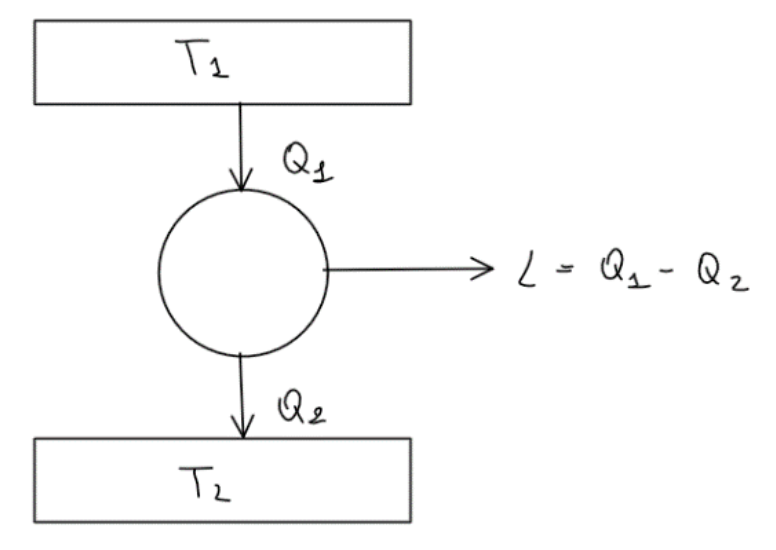
\includegraphics[width=0.3\columnwidth]{ciclomotore.png}
				\caption{Ciclo motore}
	\end{center}
\end{figure}

Otteniamo lavoro $L=Q_1-Q_2$.

Mettendo in relazione la traccia termodinamica (inverso della disugualianza di Clausius) ed il rendimento $\eta={L\over Q_1}={1-{Q_2\over Q_1}}$ otteniamo il rendimento del ciclo motore irreversibile 
\begin{equation}
	\eta=\left(1-{T_2\over T_1}\right)-\left. \tau T_2\over Q_1\right.
\end{equation}

Il primo termine corrisponde al rendimento massimo, ovvero quello di una macchina di Carnot (trasformazione reversibile, $\tau =0$).

\subsubsection{Macchina di Carnot}\index{Ciclo motore! macchina di Carnot}

È reversibile ($p_1=p_2,T_1=T_2,$ no attriti).

Isoterme tra 1-2 e 3-4 (calore è l'area sottesa).

\begin{figure}[H]
	\begin{center}
		
		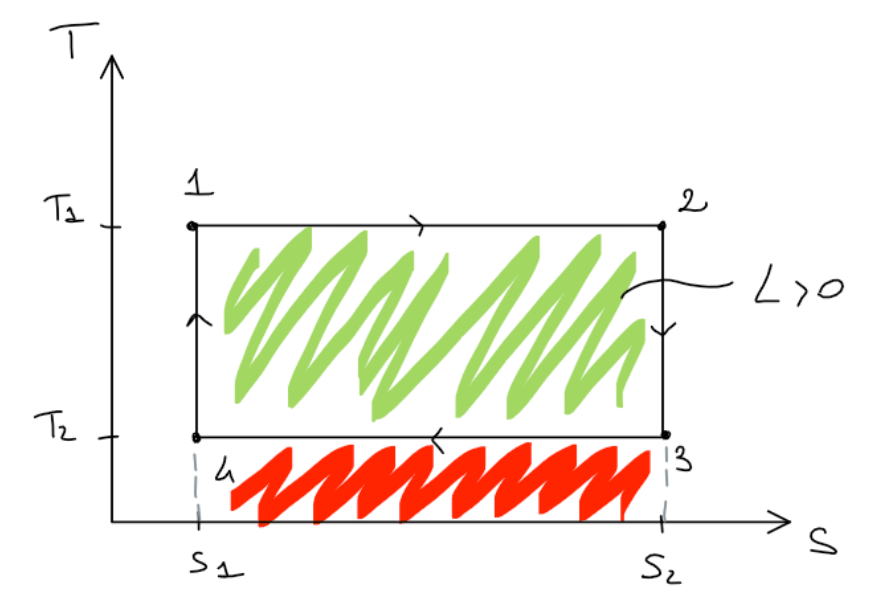
\includegraphics[width=0.4\columnwidth]{carnot.png}
		\caption{Ciclo motore}
	\end{center}
\end{figure}

Quindi abbiamo $d s=\frac{d q}{T}+d s_{S} \Rightarrow d s=0$ allora tra 2 -3 e 4-1 sono\textbf{ isoentropiche} (:=adiabatica reversibile).

È un ciclo motore particolare, infatti vale che il rendimento $\eta = \eta_c-f\left(\tau\right)$
N.B. Il rendimento di un ciclo termomeccanico massimo \textbf{non} è 1 ma $\eta_c =1-{T_2\over T_1}$

\subsection{Ciclo inverso}\index{Ciclo inverso}

\begin{itemize}
	\item ciclo frigorifero, se lo scopo è sottrarre $Q_2$ alla sorgente inferiore
	\item pompa di calore, se lo scopo è cedere $Q_1$ alla sorgente superiore
\end{itemize}


\begin{figure}[H]
	\begin{center}
		
		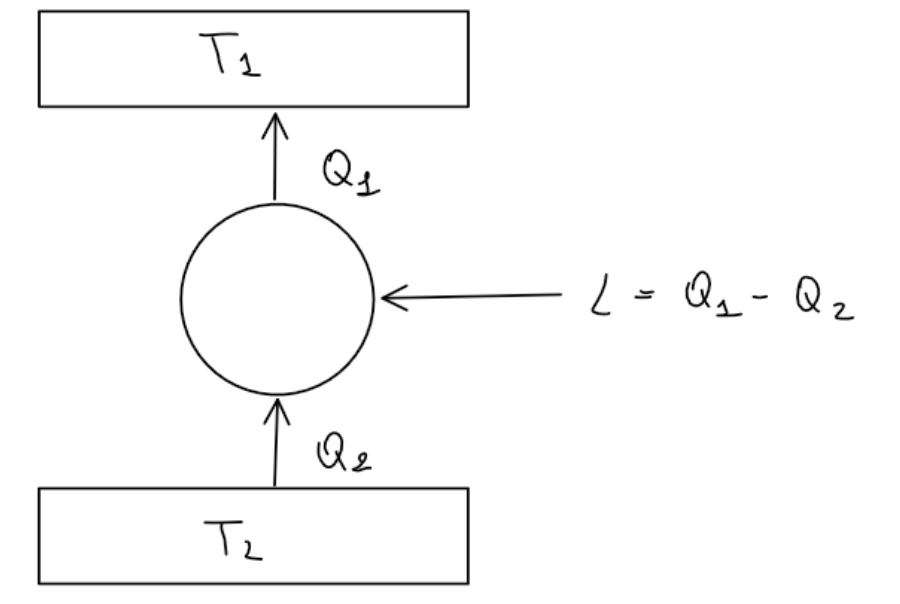
\includegraphics[width=0.3\columnwidth]{cicloinverso.png}
		\caption{Ciclo inverso}
	\end{center}
\end{figure}

\subsubsection{Ciclo frigorifero}\index{Ciclo inverso! frigorifero}
Il rendimento del ciclo frigorifero $\eta_F={Q_2\over L}=\frac{T_{2}}{T_{1}-T_{2}}-\frac{\tau}{L} \cdot \frac{T_{1} T_{2}}{T_{1}-T_{2}}$.

Il secondo termine contiene le irreversibilità.
Il diagramma nel piano Ts è un rettangolo.

\subsubsection{Pompa di calore}\index{Ciclo inverso! pompa di calore}

Il rendimento della pompa di calore $\eta_{PC}={Q_1\over L}=\frac{T_{1}}{T_{1}-T_{2}}-\frac{\tau}{L} \cdot \frac{T_{1} T_{2}}{T_{1}-T_{2}}$

Il secondo termine contiene le irreversibilità, se la trasformazione è reversibile $\tau=0$.
Il diagramma Ts è lo stesso rettangolo del ciclo frigorifero. 



\newpage
\section{Tesine}

\newpage
\section{Indici}





\listoffigures
\addcontentsline{toc}{subsection}{\listfigurename}

\newpage
\listoftables
\addcontentsline{toc}{subsection}{\listtablename}
\newpage
\listofmyequations
\addcontentsline{toc}{subsection}{\listequationsname}
\newpage
\addcontentsline{toc}{subsection}{Indice analitico}
\printindex
\newpage








\end{document}